%----------------------------------------------------------------------------
\chapter{Szoftver}
%----------------------------------------------------------------------------

\section{Felhasználói követelmények}

\begin{itemize}
	\item\textbf{Regisztráció és bejelentkezés:} Lehetőség van regisztrációra az alkalmazásban, amely után a felhasználók bejelentkezhetnek a személyes fiókjukba. Ez lehetővé teszi számukra a mentett adatokhoz való hozzáférést.

	\item\textbf{Kriptográfiai rendszerek kiválasztása:} Különböző kriptográfiai rendszerek elérhetőek, amelyeket bejelentkezés után lehet kipróbálni. Ehhez megjelenik egy menüt, ahol kényelmesen navigálhatnak a rendszerek között.

	\item\textbf{Rendszerek kipróbálása és tesztelése:} A felhasználóknak lehetősége van arra, hogy kipróbálják és teszteljék a választott kriptográfiai rendszereket. Ehhez felhasználóbarát és interaktív felületet van biztosítva, ahol megadhatják a bemeneti adatokat, és láthatják a kimeneti eredményeket.

	\item\textbf{Tanulási anyagok és információk elérhetősége:} Az alkalmazásnak tartalmaz egy tanulói felületet , ahol a felhasználók elérhetik a kriptográfiai rendszerekhez kapcsolódó részletes információkat és szemléltető anyagot. Ennek az oldalnak az eléréséhez nem szükséges a bejelentkezés.

	\item\textbf{Nyelvi támogatás:} Az alkalmazás lehetőséget ad a felhasználóknak arra, hogy különböző nyelveken használják az alkalmazást. Ehhez egy egyszerű nyelv kiválasztó van biztosítva, amely lehetővé teszi a felhasználóknak a kívánt nyelv kiválasztását. A nyelvek rövidítve, ISO 639.1-es kódjuk szerint vannak feltüntetve.
\end{itemize}

\newpage
\section{Rendszerkövetelmény}
A Cryptorithm rendszerkövetelménye funkcionális és nem funkcionális részekre oszlik. A funkcionális része tartalmazza az alkalmazás fő céljait és funkcionalitását, hogy hogyan kéne működjön a rendszer és milyen lehetőségei vannak a felhasználónak, míg a nem funkcionális rész kitér a rendszerrel szemben támasztott követelményekre, mint például a felhasználói élmény, többnyelvűség és a rendszer architektúrája.

\subsection{Funkcionális}

\begin{itemize}
	\item\textbf{Kriptográfiai eszközök:} Az alkalmazás választékot kínál a népszerű és ismert eszközökből az adatok titkosításához, visszafejtéséhez és transzformációjához. A felhasználók szabadon válogathatnak és kipróbálhatnak különböző lehetőségeket.

	\item\textbf{Tanulói felület:} Az alkalmazás rendelkezik egy tanulói felülettel, ahol a felhasználók elmélyülhetnek a kriptográfiai rendszerek megértésében. Itt információkat olvashatnak és gyakorlati példákon keresztül elsajátíthatják ezeket a rendszereket.

	\item\textbf{Többnyelvűség:} Az alkalmazás támogatja a többnyelvűséget, így elérhetővé válik idegen nyelvű felhasználók számára is. A felhasználók kiválaszthatják az anyanyelvüket vagy egyébb preferált nyelvet az alkalmazás használatához.

	\item\textbf{Visszajelzés:} Amennyiben ismert kivétel keletkezik a rendszserben ezt felugró üzeneten keresztül van leközölve, ami ismerteti a hibát. Kivétel keletkezhet nem megfelelő beviteli adatok nyomán, például rossz vagy nem megfelelő kulcsméret megadása, vagy olyan oldalra való navigáció ahova a felhasználónak nincsen jogosultsága. Az előző esetet a hibának megfelelő üzenettel közlődik, míg utóbbi egy az érvényben levő jogosultságnak megfelelő oldalra navigálja a felhasználót.

	\item\textbf{Szerepkörök:} A rendszert két fajta felhasználó számára elérhető, bejelentkezett és nem bejelentkezett. A bejelentkezett felhasználónak elérhető a weboldal összes funkcionalitása, ezzel szemben a nem bejelentkezett felhasználó nem jogosult a kriptográfia rendszerek használatára.
\end{itemize}

\begin{figure}[!h]
	\centering
	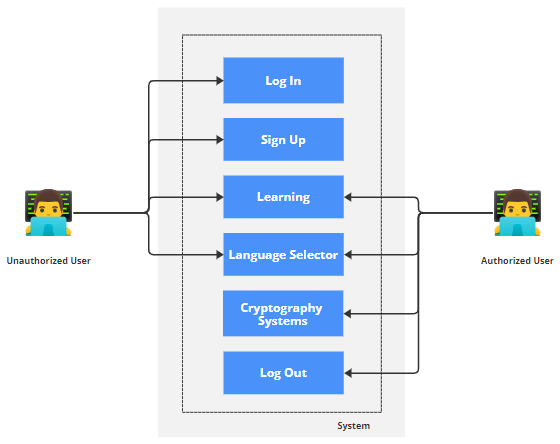
\includegraphics[scale=0.6]{images/UseCaseDiagram}
	\caption{Use case diagram}
\end{figure}


\newpage
\subsection{Nem funkcionális}

\begin{itemize}
	\item\textbf{Felhasználói élmény:} Az alkalmazás könnyen használható felhasználói felülettel rendelkezik. Az intuitív navigáció és a felhasználóbarát tervezés lehetővé teszi a felhasználók számára a könnyű kezelést és a zökkenőmentes interakciót az alkalmazással. Továbbá megfelelő felugró üzenetekkel jelez vissza a rendszer minden művelet elvégzése után.

	\item\textbf{Teljesítmény:} Az alkalmazás működése gyors és hatékony. Az oldalak betöltése és az adatbázis lekérdezések időigénye egyáltalán vagy csak enyhén észlelhetőek. 

	\item\textbf{Biztonság:} Felhasználói adatok védve vannak, megfelelően vannak tárolva. A felhasználók jelszava SHA-256-os hash formájukban vannak eltárolva az adatbázisban, valamint a kulcsok és inicializáló vektorok kigenerálása a kritériumoknak megfelelő.

	\item\textbf{Skálázhatóság:} Az alkalmazás képes kezelni a megnövekedett felhasználói forgalmat és rugalmasan skálázódni. Szükség esetén növelhetőek az erőforrások, például adatbázis kapacitása vagy a processzor teljesítménye.

\pagebreak
	\item\textbf{Hibatűrés:} Hibakezelés és hibajavítás mechanizmusainak megléte, az alkalmazásnak ellenálló képessége van a hibákhoz. Redszer leállás esetén az újraindítás nem időigényes. Az ismert, egyedi vagy lehetséges hibafaktorokra a megfelelő reakciók biztosítása, például nem megfelelő paraméterek megadása esetén hibaüzenetek kiírása és kivételek kezelése.

	\item\textbf{Kompatibilitás:} A weboldal felülete főként asztali számítógépek, laptopok képernyőjére van optimalizálva, továbbá támogatja a népszerű böngészőket.
\end{itemize}

\begin{figure}[!h]
	\centering
	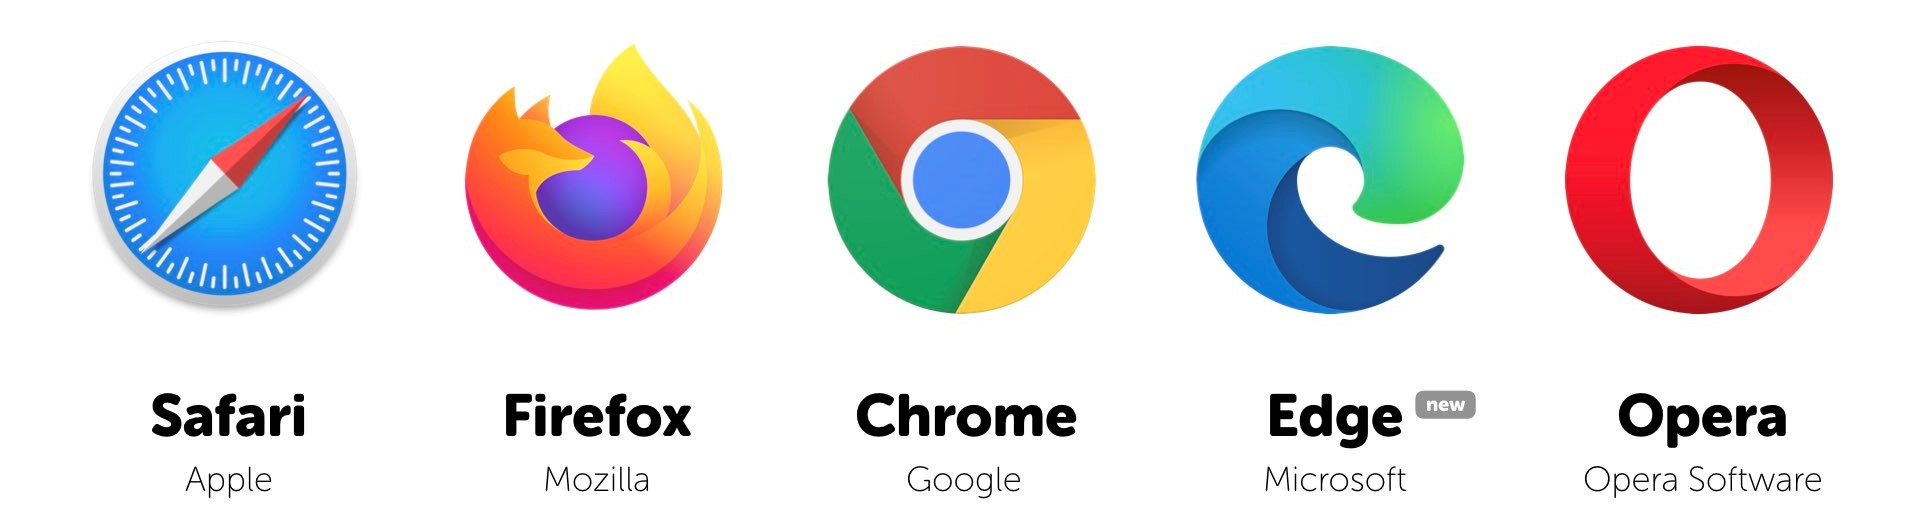
\includegraphics[scale=0.12]{images/webBrowsers}
	\caption{Népszerűbb Böngészők}
\end{figure}

\newpage
\section{A rendszer architektúrája}
Az alkalmazás architektúrája a következő komponenseket kombinálja, hogy a felhasználók kényelmesen használhassák a Cryptorithm alkalmazást. A felhasználói interfész réteg lehetővé teszi a felhasználók interakcióját az alkalmazással, az üzleti logika réteg hajtja végre a szükséges műveleteket és feldolgozza a kéréseket, míg az adatbázis réteg biztosítja az adatok tartós tárolását és kezelését. Az architektúra segít a rendszer komponenseinek szétválasztásában és a fejlesztés hatékonyságának növelésében.

\begin{figure}[!h]
	\centering
	\includegraphics[scale=0.23]{images/RendszerArchitektúra}
	\caption{Rendszer Architektúra}
\end{figure}

\textbf{Felhasználói interfész:} Ez a rész felelős az alkalmazás felhasználói felületének megjelenítéséért és a felhasználóval való interakcióért. Megvalósítása az alkalmazásban HTML, CSS és JavaScript segítségével van kivitelezve. Ez a réteg jeleníti meg a kriptográfiai rendszerek kiválasztására, tesztelésére és a tanulói anyagokhoz való hozzáférésre szolgáló felületeket.

\textbf{Üzleti logika:} Az üzleti logika réteg felelős az alkalmazás működéséért, a felhasználók által végrehajtott műveletek feldolgozásáért és az eredmények előállításáért. Itt találhatóak a szerveroldali Python fájlok, amelyek a kriptográfiai műveletek, adatfeldolgozás és adatbázis-interakciók végrehajtásáért felelősek. Flask keretrendszert használva ez a réteg kezeli a HTTP kéréseket és válaszokat.

\textbf{Adatbázis:} Az alkalmazás adatbázisában tárolódnak a felhasználói adatok, például a regisztrált felhasználók adatai és előzményei. Az adatbázis kezelésére az SQLAlchemy Python könyvtárat használtam, amely lehetővé teszi a könnyű adatbázis-műveletek végrehajtását és az adatmodell definiálását.


